\chapter{Introduction}

\section{White Dwarf Mergers}
\label{sec:wdmergers}

\subsection{The Panopoly of Stellar Mergers}
\label{ssec:stellarmergers}

Approximately two out of every three stars are born into a binary system.  A substantial fraction of these stars will interact, some due to their orbital separation at birth, while others following the expansion of one or both constituent stars as they evolve off of the main sequence.  These interactions primarily take form as mass transfer between the stars \citep{yung05}, and if mass transfer becomes unstable (increases exponentially over time), it ends with the violent coalescence of the two stars into one.  These stellar mergers, like other forms of binary interaction, disrupt single star evolution and create merged products, or ``merger remnants'', with unusual properties including blue stragglers (eg. \citealt{andrpt06, knigs09}), luminous blue variables \citep{justpv14}, subdwarf OB and R Coronae Borealis (RCrB) stars.

Mergers also liberate tremendous amounts of energy and eject significant amounts of mass, giving rise to a cornucopia of electromagnetic (and gravitational-wave) transients ranging from luminous red novae (from the merger of two (post-) main-sequence stars; eg. V838 Monocerotis and V1309 Scorpii \citep{tyle+11, nandil14}) to short gamma-ray bursts (from two neutron stars; eg. \citealt{ross15}) and the gravitational wave outburst from coalescing stellar-mass black holes (as recently found by the LIGO detector; \citealt{ligo16}).  Indeed, with current deep and short-cadence optical/near-infrared survey projects such as the Palomar Transient Factory \citep{rau+09} and Pan-STARRS \citep{kais+10} continuing to uncover more rare and even hitherto-unknown transients, and the ambitious Large Synoptic Survey Telescope \citep{lsst09} under construction, a much more complete picture of merger-generated transients will form over the next decade.

% Sec 5.2.3 of Tylenda talks about MS - MS pre-merger orbital evolution.

\subsection{Mergers of WD Binaries}
\label{ssec:c1_wdmergers_sub}

Stars with masses $\lesssim8-10\,\Msun$ generally end their lives as white dwarfs (WDs).  On their own, WDs are usually inert: held up against gravity by electron degeneracy pressure (eg. \cite{kippww12}, Ch. 15) and having ceased nuclear fusion, they will slowly radiate away their remaining thermal energy over billions of years if left alone.  WDs in interacting binaries, on the other hand, can receive mass and energy from their stellar companion, leading to a whole host of energetic and potentially explosive phenomena.

\subsubsection{The Formation of Double White Dwarf Binaries}

One common end-product of binary evolution is a pair of white dwarf (WDs).    These binaries are formed as a result of at least two phases of mass transfer (at least one of which is a common envelope event) during the binary's prior stellar evolution.  These mass transfer phases act to sap the orbital angular momentum of the 

%http://adsabs.harvard.edu/abs/2008MNRAS.387.1693C

%(Weidemann 2000, A&A 363, 647;
%Catalan et al. 2008, MNRAS 387, 1693)
%Toonen and Mennekens pop synth codes

\begin{figure}
\centering
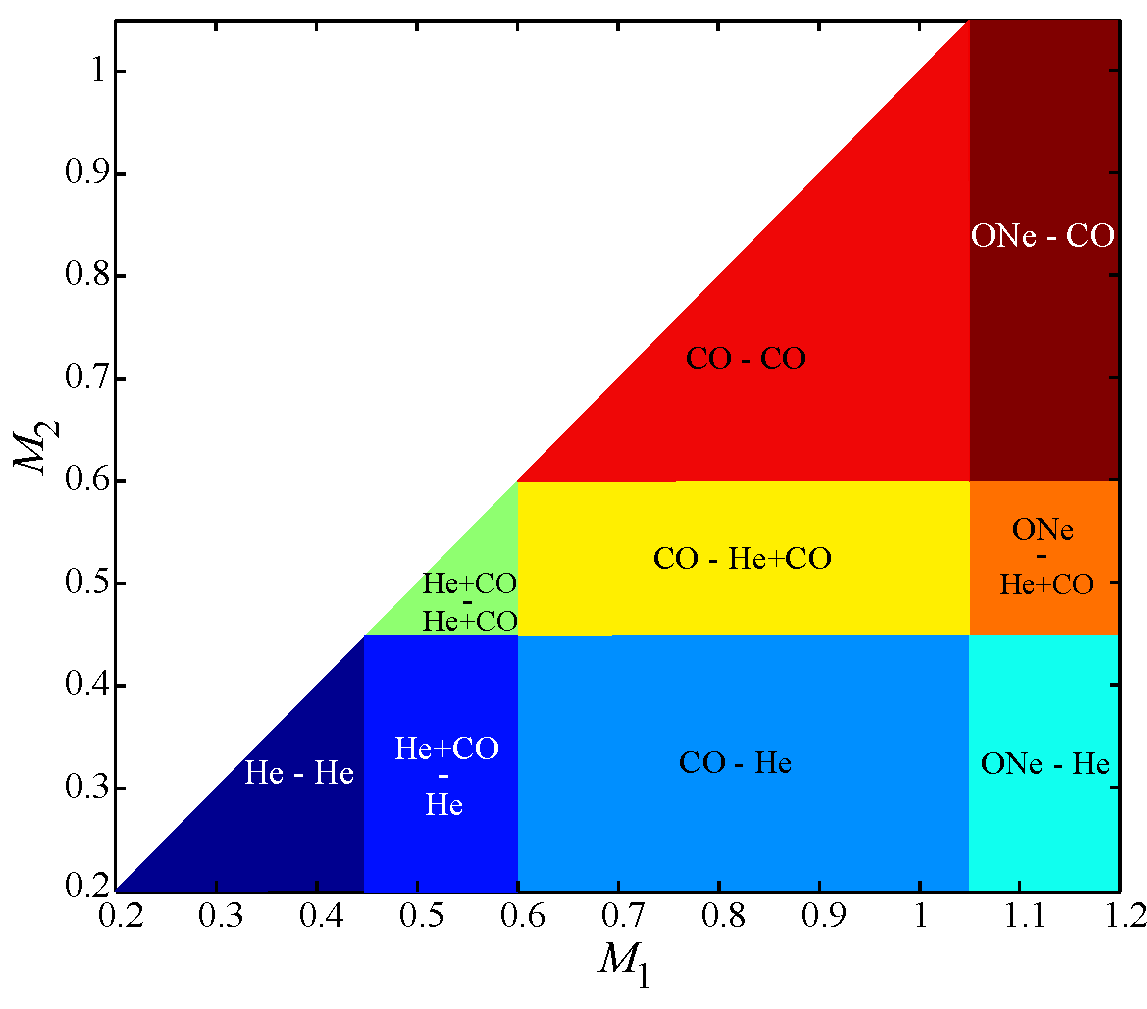
\includegraphics[width=0.6\hsize]{introduction/figures/dan+12_wdbinmass.pdf}
\caption{The mass parameter space of double WD binaries, subdivided by the dominant chemical compositions of the WDs, from \cite{dan+12}, their Fig. 1.  $M_1$ is the mass of the primary, or accreting, WD, and $M_2$ is the mass of the secondary, which donates mass.  WDs with masses $M<0.45\,\Msun$ are assumed to be He WDs, those with $0.45 < M < 0.6\,\Msun$ CO WDs with $\sim0.1\,\Msun$ He envelopes, $0.6 < M < 1.05\,\Msun$ CO WDs, and $M>1.05\,\Msun$ ONe WDs.  See text, as well as \cite{dan+12}, Sec. 2, for discussion on these choices.}
\label{fig:c1_wdbinarymasses}
\end{figure}

The mass and composition of each WD within the binary are dependent on the binary's prior evolution, and therefore are related to one another.  Broadly speaking, WDs with masses $M \lesssim 0.45\,\Msun$ are composed of helium (He), since these come from stars that had their evolution interrupted by binary interaction while on the RGB (eg. \citealt{marsdd95, nele+01, nele+01a}), before their degenerate He core became massive enough to trigger a helium flash (eg. \cite{kippww12}, Ch. 33.4).  (They could in principle also come from single stars of $\lesssim0.5\,\Msun$, but the universe is not old for any He WD to have been born this way {\charles CITATION}.)  WDs with slightly higher masses have He envelopes surrounding cores composed of carbon and oxygen (CO); \cite{dan+12} approximate the mass range of these ``hybrid WDs'' to be $0.45 \lesssim M \lesssim 0.6\,\Msun$.  From $0.6 \lesssim M \lesssim 1.1\,\Msun$ WDs are almost entirely composed of CO, with He atmospheres of $\sim10^{-2}\,\Msun$ (eg. \citealt{ibent85}).  WDs with masses $\gtrsim 1.1\,\Msun$ come from super-AGB stars (eg. \citealt{herw05}) that ignite carbon during their evolution (eg. \citealt{garc13}), and thus are composed at least partly of oxygen and neon (ONe).  

Fig. \ref{fig:c1_wdbinarymasses}, from \cite{dan+12}, summarizes these relationships for the WD binary parameter space -- in it, $M_1$ is the mass of the (more massive) primary WD, which accretes mass during the merger, and $M_2$ is the mass of the secondary, which donates mass (Sec. \ref{ssec:stable_mass_transfer}).  While nature is not so clear-cut (eg. \citealt{ibent85, moros09} for CO WDs with $M\lesssim0.45\,\Msun$), these relationships are used as rules of thumb for setting WD composition for a wide range of works (\citealt{loreig09,rask+12,dan+12,dan+14,}, with slight variations between different research groups) for setting the composition).  In this thesis, we generate binaries of CO WDs with masses ranging from $0.4 - 1.0\,\Msun$ for our parameter space study of mergers in Ch. \ref{ch:ch2}.  In subsequent chapters, we are primarily interested in the the merger of two CO WDs near the median mass of field WDs, $\sim0.65\,\Msun$ (Sec. \ref{ssec:cowd_massrange}).

The ratio of carbon and oxygen within CO WDs is also not particularly well-known.  In this thesis, we make the assumption that they are composed of 50\% carbon and 50\% oxygen by mass.  {\charles ADD STUFF}

\subsubsection{Orbital Angular Momentum Loss and Gravitational Wave Emission}

Following their formation, these binaries can lose orbital angular momentum through a number of of mechanisms, including gravitational radiation (eg. \citealt{XXX}), magnetic braking \citep{XXX} or the influence of a third body (eg. \citealt{katzd12}).  {\charles TIDAL EFFECTS?}  In the absence of a magnetized wind or third body, gravitational radiation is generally thought to be the dominant driver of angular momentum loss, and has a characteristic timescale of \citep{segrcm97}

\eqbegin
\tau_{\mrm{grav}} = 5 \times 10^5 \left(\frac{a}{10^5 \mrm{km}}\right)^4 \frac{\Msun}{\Ma} \frac{\Msun}{\Md} \frac{\Msun}{\Mtot}\,\mrm{yr}.
\label{eq:c1_gravtimescale}
\eqend

\noindent From this, we see that WD binaries with orbital periods on the order of hours or less will merge within a Hubble time.  It is estimated that there are on order of $10^8$ such systems in the Milky Way alone \citep{nele+01a,mars11}.  {\charles CHECK THESE VALUES!}

While inspiralling WD binaries with periods on the order of minutes are too low-frequency to be detected by Advanced LIGO (Laser Interferometer Gravitational-Wave Observatory \citealt{ligo+15}), they are expected to be the most numerous and dominant source of gravitational waves \citep{mars11} detected by the proposed spaceborne detector eLISA (evolved Laser Interferometer Space Antenna; \citealt{amar+13}), which probes the mHz frequency range.  Individual signals from thousands of WD binaries that are $\sim1\,\mrm{Myr}$ prior to merger can be individually resolved with eLISA \citep{amar+13,loreig09, dan+11}, while the numerous sources further away and at at longer orbital periods (lower frequencies) will comprised an unresolved background \cite{neleyp01,amar+13}.  Both of these will probe the WD binary population of the Milky Way without the selection biases that often trouble electromagnetic binary searches \citep{mars11}.  {\charles Note, however, that final coalescence of the WDs is over far too quickly to be detectable by eLISA.}  The energy lost to gravitational radiation also plays a negligible role during the merger, being is $\sim10^{-10}$ of the binary's binding energy (eg. \citealt{loreig09}).

\subsubsection{Merger Outcomes}

Like any merger, those between WDs liberate tremendous amounts of energy.  This can lead to enough heating and/or compression to reignite the nuclear furnaces of normally inert WDs under either non-degenerate or degenerate circumstances.  As such, the end product of such mergers are diverse, ranging from stars with unusual properties undergoing stable nuclear burning to explosions. Hydrostatic (and non-rotating, unmagnetized {\charles CITATION}) WDs have a maximum stable mass beyond which bodies supported by electron degeneracy pressure are unstable to collapse.  This is known as the \cite{chan31} mass, or \Mch, and is at $\sim1.4\,\Msun$.  This has long led to the notion that sufficiently massive WD mergers can lead to the complete destruction of the merger product, either in a thermonuclear explosion that would resemble type Ia supernovae (SNe Ia; \citealt{webb84}), or transformation into a neutron star (NS) in an event known as an accretion-induced collapse \citep{nomoi85, saion85}.  Today, however, we know of a much greater range of possible merger outcomes, both for binary systems with masses above and below \Mch.  Which outcome occurs depends largely on the compositions of the WDs involved, and are briefly summarized below (see also \citealt{dan+14}, who produce a similar list):

% dan+14 Fig 12, dan+12 fig 8

\begin{itemize}
	\item The merger of {\bf two He WDs} is unlikely to lead to violent nuclear burning and an explosion \citep{dan+12,dan+14,dan+15}.  Instead, merger remnants with total masses $0.4\lesssim \Mtot \lesssim 0.8$ \citep{han+02,pacz71}\footnote{This is lower than the He flash mass of $\sim0.45\,\Msun$ because the merger remnant is partly non-degenerate \citep{han+02}.}, which are the vast majority of double He WD remnants \citep{nele10}, are expected to ignite He burning in a shell \citep{saioj00,zhanj12}.  This increases the radius and luminosity of the star until it becomes a yellow giant after $\sim 10^3-10^4\,\mrm{yr}$, with properties similar to extreme helium (EHe) and R Coronae Borealis (RCrB) stars {\charles \citep{saioj00, zhanj12}.}  Over the next $10^5-10^6\mrm{yr}$, the burning shell migrates inward with a series of weakening shell flashes, while the radius slowly shrinks to $\sim10^{-1}\,\Rsun$.  Once the shell reaches the center of the remnant, stable He fusion is ignited, and remnant settles onto the helium main sequence, resembling a subdwarf B or O star \citep{saioj00, justph11, zhanj12}.  While most subdwarf stars are in binaries, and likely form from other formation channels channels, mergers are expected to be a major -- perhaps even the main -- source of single subdwarf stars (eg. \citealt{han+03, nele10}).

	\item The outcome of a merger betwee {\bf an He and a CO WD}, or a merger between an He and hybrid He-CO WD, depends on whether or not a He detonation is touched off during the merger.  The conditions for which either occur remains a field of active research (eg. \citealt{holc+13, shenm14, dan+15}).  Roughly speaking, mergers with $\Mtot \lesssim 0.8\,\Msun$ are unlikely to trigger a detonation and will instead ignite He burning in a shell; they have been proposed as the progenitors to He-rich sdO stars (\citealt{justph11}; He-poor sdO stars are likely evolved sdB stars).  Mergers with $\Mtot \gtrsim 0.8\,\Msun$ that do not detonate will also ignite shell burning, but unlike sdOB progenitors they will retain their extended envelope for the duration of their burning phase \citep{pacz71}.  These mergers are believed to be the primary formation channel for R CrB stars \citep{webb84, clay+07, clay12, kararh15}, which are H-deficient, He- and C-rich supergiants that feature abrupt variability by up to a factor of $\sim10^3$ due to the formation of carbon dust above their photospheres.

Helium detonations become more likely for binaries with $\Mtot\gtrsim\Mch$ \citep{dan+14, dan+15}.  For extremely 

%The conditions under which He will detonate, and whether this detonation proceeds to disrupt or destroy its host star, is a field   While it is difficult to say whether these conditions can be achieved during a merger \citep{dan+15}, if an explosion did occur, He will not burn to nuclear statistical equilibrium, and the resulting ejecta will be composed largely of a mixture of intermediate-mass elements such as Ca, Ti and Cr.  See below.

	\item The merger of {\bf two CO WDs} has long been suspected of producing an SN Ia under the right conditions (Sec. \ref{sec:mysteryofsneia} and \ref{sec:vkchannel}).  If these conditions are not met, they will instead create a lone massive, rotating and highly magnetized CO WDs or, if steady carbon fusion is ignited, a carbon-burning star that eventually turns into an ONe WD (Sec. \ref{sec:hotdqs}).  If the ONe WD is above \Mch, it may experience an AIC (see below).

	\item Mergers where the accretor is an {\bf ONe WD}.  \cite{dan+14} also discusses the possibility of ``hybrid supernovae'', where 

\end{itemize}

Of these possibilities, it is the CO - CO WD mergers that have been most 

%The outcome of a merger between a CO (or hybrid CO-He) WD and an He WD depends on whether or not a detonation is touched off during the merger, and if this detonation is then able to propagate into the accreting WD's core and trigger a second detonation which destroys the accretor (or possibly both stars).  The conditions for which either occur is a field of active research (eg. \citealt{holc+13, shenm14, shenb14, dan+15}) which is beyond the scope of this thesis.  Roughly speaking, however, He detonation is much more likely to occur in merging binaries with \Mtot\ close to or above \Mch\ \citep{dan+14}.

%Mergers whose total mass $\Mtot\lesssim0.8\,\Msun$ will produce remnants that subsquently ignite He burning in a shell, and evolve in a manner similar to their less massive He - He WD remnant cousins, and have been proposed as the progenitors to He-rich sdO stars \cite{justph11}.  Mergers with $\Mtot\gtrsim0.8\,\Msun$ will retain their expanded envelope for much longer \cite{pacz} and become He giants.  This is believed to be the main channel to produce extreme helium and R Coronae Borealis stars \citep{xxx}.  


%%\cite{clay+07} semi-analytically calculate disk accretion following a merger between a CO WD of variable mass and an He WD of either 0.2 or 0.4 {\Msun}.  They state that accretion occurs at an average rate of $\sim 30$ - $140$ {\Msun} yr$^{-1}$ (assumed to be steady over time), building up an He atmosphere.   The temperature of the atmosphere, $1$ - $4 \times 10^8$ K, is high enough to ignite He, and significant nuclear processing results (without explosion, in line with Sec. \ref{ssec:mechanicsofwdmergers}) \citep{clay+07}.  \citeauthor{clay+07} suggest that ``hot'' (with nuclear burning) mergers between He WDs and CO WDs will form hydrogen-deficient (HdC) and R Coronae Borealis stars.  This is qualitatively suggested by the extremely low isotopic ratio of $^{16}$O/$^{18}$O $\lesssim 1$ (less than 0.2\% solar), indicating significant production of $^{18}$O.  \citeauthor{clay+07} perform a nucleosynthesis experiment simulating He burning on the merger remnant atmosphere, and recover similar isotopic ratios as are observationally found in RCrB stars.

%%\cite{saioj02} also model the post-merger evolution of a remnant formed by a 0.5 - 0.6 {\Msun} CO and a 0.1 - 0.4 {\Msun} He WD, assuming a mass accretion rate of $10^{-5}$ {\Msun} yr$^{-1}$.  Like the He-He merger remnants in \cite{saioj00}, once He burning begins the system evolves toward a yellow giant, during which a series of weak He flashes will occur.  Depending on how much He exists above the shell, the star will remain as a yellow giant for some time, before He exhaustion moves the star toward the blue side of the HR diagram.  The blueward evolutionary track of the giant on a log g vs. log T$_{\mathrm{eff}}$ passes by the values of a number of observed EHes.  Additionally, luminosities, masses, secular evolution and (broadly) surface compositions of observed EHes can be explained by this formation channel.  The rate of CO-He mergers (as given by \cite{nele+01a}) and the time period over which a remnant will appear to be an EHe combined give a of EHes in the Milky Way that roughly matches the observed number.  This suggests that CO-He mergers are the primary progenitor to EHes, and a sizable number of CO-He mergers are quiet.

%%%\cite{saioj00} note that HdCs and RCrB stars are similar in luminosity and surface composition to EHes (without any nucleosynthesis during the merger), but are cooler, and so they consider their merger model to be equally applicable to HdC and RCrB star formation.  


%As shown above, if accretion rates for the disk onto the merger remnant are above $\sim 10^{-5}$, hydrostatic burning ensues.  If, however, accretion rates are below $\sim 10^{-6}$ {\Msun} yr$^{-1}$, a He thermonuclear explosion could result that disrupts the outer He layer of the star.  If this event is a detonation, known as a ``.Ia supernova'', the detonation wave may even travel into the CO core, producing a second, carbon-oxygen, detonation.  Accretion rates are critically dependent on the viscosity of the thick post-merger disk.  Based on estimates from \citeauthor{loreig09} of the viscous timescale, core accretion could as low as $10^{-10}$ - $10^{-14}$ {\Msun} yr$^{-1}$ if the viscosity is laminar, or as high as $10^2$ {\Msun} yr$^{-1}$ if viscosity is turbulent.  If we entertain the possibility of very low viscosity rates, then a He envelope disruption becomes much more likely.

%\cite{guil+10} suggests another possible explosion channel.  During the merger itself accretion rates ranging from $10^{-5}$ - $10^{-2}$ {\Msun} yr$^{-1}$ will result in shearing within the accreted He envelope, which then creates large-scale Kelvin-Helmholtz instabilities.  These instabilities form over-dense regions that periodically compress the inner regions of the envelope, possibly resulting in conditions for detonation.  Using the results of SPH simulations, \cite{guil+10} simulate unstable WD binary mass transfer in an adaptive mesh code, and find detonation may be possible on a (0.6 - 0.9 {\Msun}) CO WD that has accreted $~sim$ 0.1 {\Msun} of He.  \citeauthor{guil+10} did not study if this process could also occur during post-merger disk accretion.

%\subsubsection{He Novae and Deflagrations}

%\cite{woosk10} carry out an extensive investigation into He shell detonations, including the conditions within the He shell necessary for detonation.  An explosion will occur so long as the dynamical timescale is longer than the nuclear timescale.  Whether this explosion is a helium nova, or a deflagration or detonation of the entire shell, depends on the convective timescale compared to the ''runaway timescale''.  \citeauthor{woosk10} define the runaway timescale as the time it takes for He (with its current temperature) to rise to extremely high temperatures if convection were artificially turned off.  From their simulation results, they take $\tau_{\mathrm{run}} \approx 2$ s to be a good trace of the boundary between nova and detonation/deflagration, which they translate to a relationship between density and pressure.  Similarly, to form a detonation shockwave via the Zel'Dovich mechanism requires that the ratio of distance between two points over the difference in their nuclear runaway timescales be larger than the sound speed to create a detonation wave.  This translates to (using the assumption of adiabaticity of the temperature gradient) a relationship between density and temperature, which is plotted alongside simulation results in Fig. \ref{woosleyfig}.  Simulations show that these semi-analytical estimates should be trusted only to first order.

%\begin{figure}
%\centerline{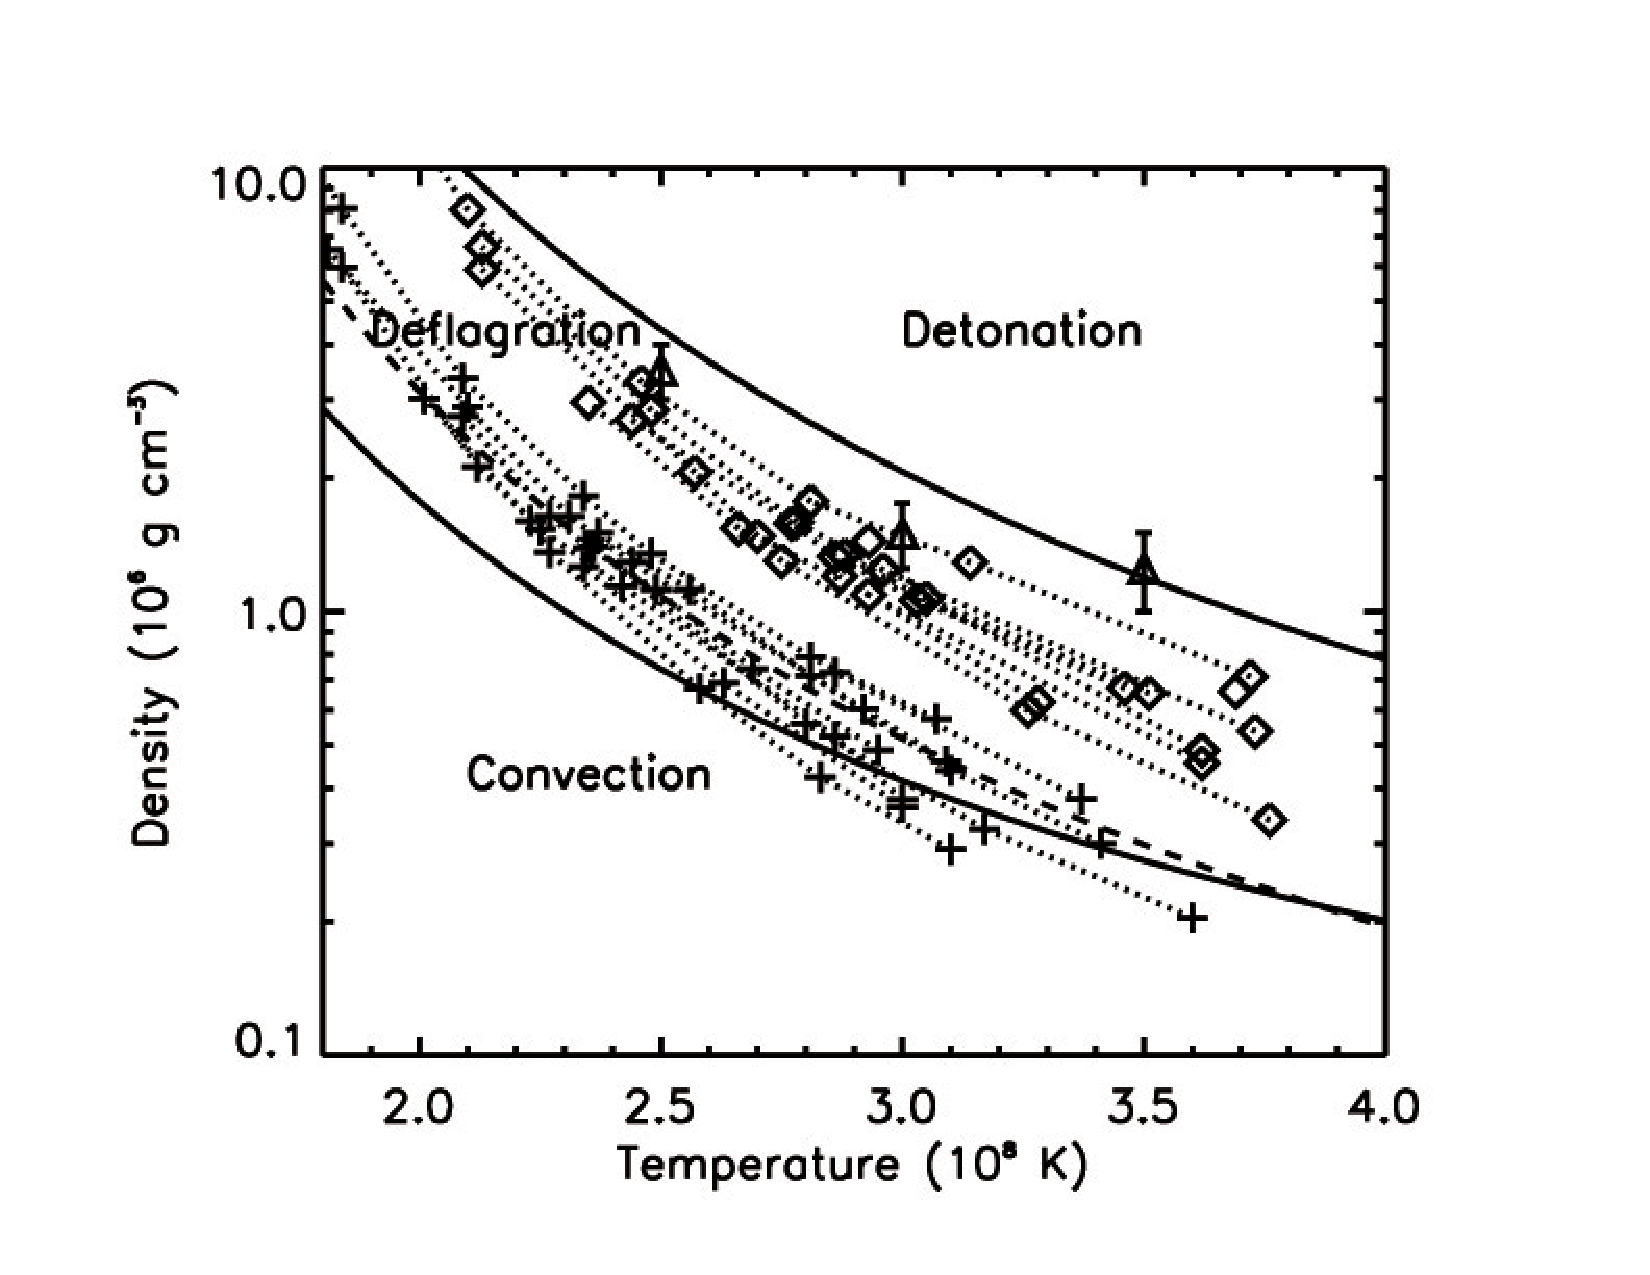
\includegraphics[width=1.0\hsize]{woosleyfig.pdf}}
%\caption{A plot of density versus temperature for the He burning region, with the regions for He novae, deflagrations and detonations indicated.  Along with the two analytic estimates of the boundaries of the different regions, a number of simulations are also plotted here.  Diamonds indicate planar (1D) simulations that eventually reach a thin burning shell luminosity of $10^{47}$ erg s$^{-1}$, and crosses indicate simulations that achieve $10^{46}$ erg s$^{-1}$.  Dotted lines connecting diamonds/crosses indicate families of simulations for which the accreting CO WD was identical, but the accretion rate is varied.  All simulations that reached $10^{47}$ erg s$^{-1}$ detonated, and most that reached $10^{46}$ erg s$^{-1}$ deflagrated.  Discrepancy between the analytic estimates and the simulations are due to simulations accounting for gas dynamics and utilizing a more correct equation of state.  Apparently, dividing the analytic deflagration-detonation border by four (arbitrary value) gives a better fit to the simulations (dotted line).  The deflagration-detonation border determined by fine-zone simulations looking single-point detonations are given by triangle points.  From \cite{woosk10}, their Fig 2.}
%\label{woosleyfig}
%\end{figure}

%Below a critical density/temperature given in Fig. \ref{woosleyfig}, convection can effectively carry away energy from the thin shell, resulting in He novae, which are covered in another section of the report.  In the intermediate region between the $\tau_{\mathrm{run}} \approx 2$ condition for explosion and the condition for detonation is the regime for He deflagrations, which are weak (peak B-band magnitude of $\sim$ -15, ejecta velocities of $\sim$ 6000 km s$^{-1}$ for unburned He, and slower for heavier elements), fast-evolving explosions that produce $\sim$ 0.1 {\Msun} of mostly intermediate-mass elements, or IMEs, ($< 10^{-4}$ {\Msun} {\Ni}) and are powered primarily by $^{48}$Cr \citep{woosk10}.  For the two deflagrations simulated by \citeauthor{woosk10}, both ejected most of the accreted He envelope, but processed very little of it.  He deflagrations are covered in another section of the report as well.

%Note that some of \cite{wald+10}'s simulations skirt perilously close to the deflagration regime, while \cite{shen+10}'s simulations have initial conditions more firmly in the detonation regime.

%\subsubsection{He Detonation Without CO Detonation (.Ia Supernova)}

%% THIS IS WRONG: A merger between a {\Msun} CO WD and a lower-mass {\Msun} He WD will result in a cold CO core surrounded by a hot He envelope and disk.  If the disk subsequently accretes onto the remnant core at the prodigeous rates suggested by \citeauthor{clay+07} and \citeauthor{loreig09} (their turbulent viscosity rates), it is conceivable that compressional heating will drive the base of the He core to high enough temperatures and densities to detonate, (see Sec. \label{ssec:withcarbon-oxygencompanions} for a similar argument for CO WDs).  Alternatively, hot-spots created during the merger may reach similar conditions (\textit{a la} \citeauthor{pakm+10}'s CO-CO merger situation) and detonate.

%\cite{woosk10}, \cite{shen+10} and \cite{wald+10} all simulate in 1D detonations at the base of the merger remnant He envelope, with CO burning artificially supressed, and all find the detonation unbinds the entire He outer layer of the remnant, while the CO layer is left relatively intact.  Of these, \citeauthor{wald+10} is particularly interesting due to the higher mass ratio between the CO core and He shell (which would more likely for a merger).  \citeauthor{wald+10} explore a range of CO core (0.45 - 0.6 {\Msun}) and He envelope (0.15 - 0.3 {\Msun}) masses and find that, for those detonations above CO cores below 0.6 {\Msun}, explosions produce large quantities of $^{40}$Ca, $^{44}$Ti and $^{48}$Cr, and very little {\Ni}.  For a given CO core mass, the mass fraction in the ejecta of {\Ni} increases with the mass of the He shell.  Additionally, {\Ni} mass fraction can be reduced by polluting the remnant's envelope with CO - at $\sim 10^8$ K, $\alpha$ capture onto carbon is faster than the $\alpha$ process, allowing carbon to effectively slow the nuclear reaction rate of He.  Simulated light curves have a rise time of $\sim$ 7 days, a $\sim$ -11 to -18 peak bolometric magnitude, and highly differing late-time behaviour, depending on the mix of radioactive species produced.

%\cite{shen+10} and \cite{woosk10} also simulate He shell detonations in 1D, focusing on detonating thin ($\sim$ 0.02 - 0.1 {\Msun}) He shells on top massive cores (0.6 {\Msun} CO - 1.2 {\Msun} ONeMg) to simulate .Ia SNe.  \citeauthor{shen+10}, however, also simulate detonations of 0.2 - 0.3 {\Msun} envelopes over 0.6 {\Msun} cores, and their resulting light curves and spectra are in general agreement with those of \citeauthor{wald+10}, despite having a different code and a more realistic detonation initialization (though they also do not consider core detonations).  Resulting light curves are, again, highly varied.  As an example, in their 0.6 {\Msun} CO - 0.3 {\Msun} He detonation, 0.3 {\Msun} is ejected (of which 65\% is {\Ni}), with a average asymptotic velocity of $1.3 \times 10^{4}$ km s$^{-1}$ and kinetic energy of $5.3 \times 10^{50}$ erg s$^{-1}$.  The peak bolometric magnitude obtained is -18.  \citeauthor{woosk10} simulates the acutal He accretion process, and provide detailed analysis of the process leading from accretion to explosion.  Their simulations reproduce light curves with a range of peak values and ${\delta}m_{15}$ (number of magnitude drops 15 days after the start of the SN) similar to those found by \citeauthor{shen+10}.  Ejecta velocities and spectroscopic features are also similar between the two papers.  \cite{woosk10} also note that hotter CO WD accretors tend to produce weaker, faster explosions that resemble the He deflagrations mentioned in the previous section.

%%\cite{frye+09} simulate a .Ia in an enshrouded environment, and manage to obtain -18 as well, but why do they only get -16 in an un-enshrouded case?

%%\cite{woosk01}, \cite{shen+10} and \cite{wald+10} all simulate in 1D detonations at the base of the He envelope of such a remnant, with CO burning artificially supressed\footnote{The CO burning suppression is to prevent spurious centre-lit CO detonations arising from the assumption of spherical symmetry in the detonation shockwaves \citep{wald+10}.}.  They find the detonation unbinds the entire He outer layer of the remnant.  Of these, \citeauthor{wald+10} is interesting in particular due to the higher mass ratio between the CO core and He shell (which would more likely for a merger).  \citeauthor{wald+10} explore a range of CO core (0.45 - 0.6 {\Msun}) and He envelope (0.15 - 0.3 {\Msun}) masses and find that, for those detonations above CO cores below 0.6 {\Msun}, explosions produce large quantities of $^{40}$Ca, $^{44}$Ti and $^{48}$Cr, and very little {\Ni}.  For a given CO core mass, the mass fraction in the ejecta of {\Ni} increases with the mass of the He shell.  Additionally, they note {\Ni} mass fraction can be reduced by polluting the remnant's envelope with CO - at $\sim 10^8$ K, $\alpha$ capture onto carbon is faster than the $\alpha$ process, allowing carbon to effectively slow the nuclear reaction rate of He.  \citeauthor{wald+10}'s simulations suggest that the envelope will be unstable to convection and allow for CO dredge-up, and \citeauthor{loreig09} note appreciable amounts of C and O in the hot envelope of their 0.3 - 0.5 {\Msun} He-CO merger remnant.  Simulated light curves have a rise time of $\sim$ 7 days, a -15 to -18 peak bolometric magnitude, and highly differing late-time behaviour, depending on the mix of radioactive species produced.

%%\cite{shen+10} also simulate He shell detonations in 1D, focusing on detonating thin ($\sim$ 0.02 - 0.1) He shells on top massive cores (0.6 CO - 1.2 ONeMg) to simulate .Ia SNe.  They do, however, also simulate detonations of 0.2 - 0.3 {\Msun} envelopes over 0.6 {\Msun} cores, and their resulting light curves and spectra are in general agreement with those of \citeauthor{wald+10}, despite having a different code and a more realistic detonation initialization (though they also do not consider core detonations).  The trend of increasing {\Ni} production with increasing shell mass is reproduced in both simulations, and a 0.6 CO - 0.2 He, the one simulation common to both studies, both simulations produced comparable amounts of unburned $^4He$ and similar nucleosynthetic producs (\citeauthor{wald+10} produced more {\Ni} and less intermediate mass elements).  For their 0.6 {\Msun} CO - 0.3 {\Msun} He detonation, 0.3 {\Msun} is ejected (of which 13\% is {\Ni} and 12\% is $^{44}$Ti), with a average asymptotic velocity of $1.3 \times 10^{4}$ km s$^{-1}$ and kinetic energy of $5.3 \times 10^{50}$ erg s$^{-1}$.  The peak bolometric magnitude obtained is -18.

%%We should note that \cite{wald+10}, \cite{shen+10} and \cite{woosk10} all perform simulations detonating thin He shells over massive CO cores in order to simulate .Ia detonations; the resulting explosions also feature significant amounts of intermediate mass elements (the amount goes down as mass goes up), but much less mass is ejected, and in general peak light is much dimmer with a faster rise time.

%%THIS IS WRONG \footnote{While \citeauthor{shen+10} having significantly more unburned He than \citeauthor{wald+10} should have an effect on He absorption line strengths, but because neither code accounts for non-local thermal equilibrium (``non-LTE'') effects such as non-thermal electron excitation caused by Compton scattering of $\gamma$ rays (required to explain He absorption lines in Ib SNe), the differences due to unburned He are suppressed.}

%%http://texblog.wordpress.com/2007/08/28/placing-figurestables-side-by-side-subfigure/ tells you how to do this without Photoshop.

%\begin{figure}
%\centerline{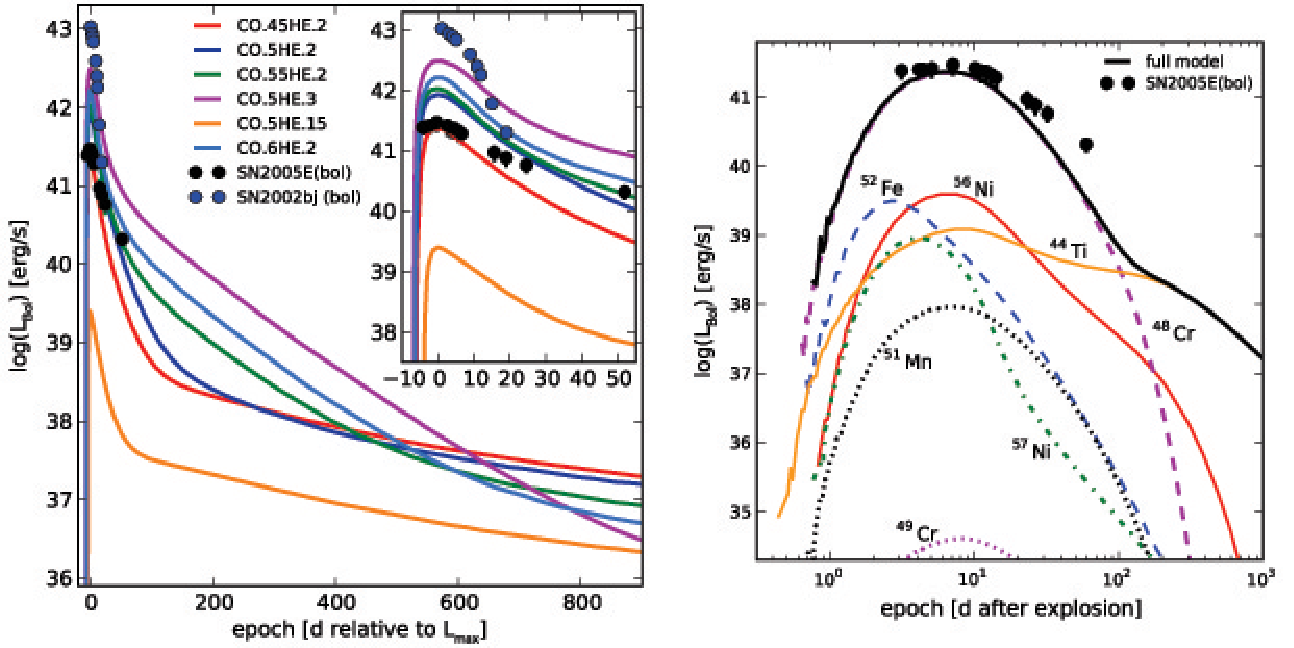
\includegraphics[width=1.0\hsize]{waldmanfigure.pdf}}
%\caption{Left: bolometric light curves of 1D explosion models simulated by \citeauthor{wald+10}, compared to type Ib SN 2005E and SN 2002bj.  Error bars of the observed SN include errors due to unobserved bands.  Right: light curve for SN 2005E compared with a 0.45 {\Msun} CO core, 0.2 {\Msun} He envelope remnant (\citeauthor{wald+10}'s best fit to SN 2005E), along with the light curve contributed by each radioactive element decay chain.  Note that at early times the light curve is dominated by $^{48}$Cr, and at late times by $^{44}$Ti.}
%\label{waldmanfigure}
%\end{figure}

%He shell detonation has been proposed as an explanation for fast, low-luminosity type Ib SNe that produce very little {\Ni}, have low ejecta masses and have moderate ejecta velocities, and spectroscopically show strong lines of He, Ca and Ti \citep{pere+10a,wald+10}.  The prototype of this class is SN 2005E, which had (assuming only {\Ni}-decay powered light curves) 0.28 {\Msun} of ejecta, 0.003 {\Ni} produced, and $1.1 \times 10^{4}$ km s$^{-1}$ average ejecta velocity \citep{pere+10a}.  While these explosions could be caused by core-collapse of $\sim$ 10 {\Msun} stars, these SNe appear from both young and old stellar populations, and debate is still ongoing regarding the environments that spawn such SNe (Ibs also typically have far greater ejecta masses and greater nucleosynthetic output) \citep{kawa+10,pere+10a,wald+10,pere+11}.  Another class of fast SN, SN 2002bj-like SNe (peak B-band light $\sim -18.5$, 0.15 {\Msun} ejected - most of it {\Ni}, on order $10^{50}$ ergs kinetic energy), has also been proposed to be caused by He shell detonations due to their correlation with older stellar populations and their low ejecta masses \citep{pere+10b}. For SN 2002bj, however, the evidence for He in the spectrum is less conclusive than for SN 2005E \citep{pere+10b, pozn+10}.

%\citeauthor{wald+10} compared their models to the light curve of SN 2002bj, and light curve and spectrum of SN 2005E.  While they cannot exactly reproduce the light curve and spectrum of SN 2005E, their 0.45 CO - 0.2 He detonation model can reproduce SN 2005E's peak-light (-15th mag) and ejecta velocities.  On the other hand, the models have faster late-time declines, and faster evolving spectra, than SN 2005E. Though most observed features are replicated by the light curve, their strengths are not.  Both facts suggest that SN 2005E had a somewhat different total ejecta mass (the model gives $\sim$ 0.2 {\Msun}; an estimate from observations assuming a light curve powered only by {\Ni} gives $\sim$ 0.28 {\Msun}) and composition.  SN 2002bj-type light curves are either too bright at peak light, or decay too quickly, to fit well to the curves of either \citeauthor{wald+10} or \cite{sim+10}, suggesting either alternative explosion mechanisms or the need for a more detailed study of He shell detonation parameter space.

%\cite{brow+11} study a sample of 12 extreme low mass (ELM; $\leq 0.25$ {\Msun}) He WDs, 11 of which are in binary systems \footnote{\citeauthor{brow+11} make the case that the 12th is likely a pole-on binary system, since low mass He WDs cannot be made through single-star evolution}.  From this sample they determine the combined merger and stable mass transfer system creation rate to be $4 \times 10^{-5}$ yr$^{-1}$ (which they note is likely an underestimate), of which they estimate, by using Eqn. \ref{qcrit2}, that $\sim 30$\% of this rate will be He-CO WD mergers, meaning the He-CO WD merger rate is $\sim 1 \times 10^{-5}$ yr$^{-1}$.  Supplementary material from \citeauthor{pere+10a} give the rate of calcium-rich SNe to be $\sim 7$\% of the total SN Ia rate, which \citeauthor{brow+11} give as $5 \times 10^{-3}$, meaning that mergers between low mass He and CO WDs only accounts for a fraction of calcium-rich SNe.  Other progenitors may include mergers involving heavier He WDs (much more common, cf. Secs. \ref{ssec:populationstatistics} and \ref{ssec:possibleexplosivenuclearburning}), He transfer from non-WD companions, or other detonation mechanisms \footnote{Including mergers of ELM He WDs with other HE WDs would approximately double \citeauthor{brow+11}'s rates.}.


%% Such mergers then contribute $\sim 10$\% of the total estimated rate of underluminous SNe, $\sim 1 \times 10^{-4}$ yr$^{-1}$ \citep{fole+09,brow+11}.  Note, however, that this last value is based on single event statistic

%%Note that the total rates \citeauthor{brow+11} give include .Ia from AM CVn systems formed from ELM WD colaescences.  Since this is not a useful number to cite for

%%A nuclear detonation of an He shell around a CO core will have a distinct signature (WHAT IS IT?).  Such events have been cited as being responsible for low-mass, low-to-normal luminosity and fast-evolving SNe.

%%Kawabata thinks it comes from a 10 {\Msun} star (2010Natur.465..326K), though a mapping of the region finds no evidence of recent star formation or a younger stellar population that could explain the origin of a 10 {\Msun} star 2011ApJ...728L..36P.

%\subsubsection{He Detonation With CO Detonation}

%If a detonation were to occur in He, it is possible for this detonation to propagate into the CO core as a edge-lit (i.e. CO-He interface-lit) CO detonation, disrupting the entire WD.  An outward propagating He detonation could also, via inward propagating shockwaves, compress the CO core to the point at which its centre ignites.  An He detonation triggering a CO detonation is known as the ``double-detonation'' scenario, and has been well-studied (cf. references in \cite{woosk10}, \cite{finkhr07} and \cite{fink+10}).  \citeauthor{woosk10} find very little difference in outcome between edge-lit and compressional double-detonations.

%A significant issue discussed by \citeauthor{woosk10} is that for a compressional detonation the inward shocks must converge in a region less than 100 km across to light the CO detonation.  Current 1D simulations artificially satisfy this convergence, but if an He detonation is to be reached the He nuclear runaway layer must fragment into small sections that do not communicate with each other, and whether a simultaneous detonation at multiple points is possible is still an open question.  A probable outcome is an asynchronous detonation of several extended regions in the runaway layer, and the resulting lack of shockwave convergence makes a CO detonation more difficult \citep{woosk10}.  An issue for the edge-lit detonation is propagation of the He detonation wave into CO core, which is a function of density, altitude of the He detonation from the CO core, and the degree of He-CO mixing at the interface between the two layers.  \citeauthor{woosk10} note that both problems require a more detailed understanding, and treatment in 3D simulations.

%MAY WANT TO DOUBLE-CHECK WITH PHIL THAT EDGE-LIT DOESN'T REQUIRE CONVERGENCE.

%\cite{finkhr07} perform 2D simulations (z-axis vs. radius coordinates) of compressional detonations from various initial flame geometries, such as single point detonations, spherical shell detonations, and single/multiple torus detonations.  Their initial system consists of either a 0.8 {\Msun} CO core with a 0.2 {\Msun} He shell, or a  0.9 {\Msun} core with a 0.1 {\Msun} shell.  They also followed up a single point detonation using a full 3D cartesian simulation.  They find that the majority of their detonations result in a secondary core explosion, and they argue that due maximum density being resolution limited, it is likely all their simulations should lead to explosions if their resolution was infinite\footnote{This is due to the fact that \citeauthor{finkhr07} find that all of their initial flame geometries eventually produce inward propagating shocks that are roughly spherically symmetric - this symmetry has an amplification effect on the shock.}.  Their explosions are comparable to (though somewhat weaker than) normal SNe Ia: all 1.0 {\Msun} are ejected, with an average speed of $\sim 10^4$ km s$^{-1}$, and $\sim$ 0.4 {\Msun} {\Ni} is produced.  Their 3D result is very similar to their 2D results, only producing 0.05 {\Msun} more {\Ni}.  Follow-up work (still in 2D) was presented in \cite{fink+10} with a refined nuclear reaction chain.  The results from \cite{finkhr07} still hold, except that more of the He shell burned into IMEs during the explosion rather than {\Ni}, which would help make the explosion look more like an SN Ia (see below).  Again the entire star is ejected, about 0.2 - 1.1 {\Msun} of {\Ni} is produced (highly dependent on progenitor mass) and 10$^{51}$ ergs asymptotic energy is released.  These results has been challenged by \citeauthor{woosk10}, who state that \citeauthor{fink+10} uses a completely convective envelope, while their simulations of comparable initial masses, using more correct initial conditions where convection is frozen-out, burn He all the way to {\Ni}.  Note that \cite{finkhr07} and \cite{fink+10} use perfect mirror symmetry and assume complete burning from He to Ni during explosions, both somewhat unrealistic assumptions that significantly increase the chances of detonation \citep{guil+10}.

%Traditionally double-detonations have been contenders for SN Ia progenitors.  Model spectra from such events, however, do not match spectra of observed SN Ia - IME lines are too weak in the models, owing to the nuclear processing of the outer He layer to {\Ni} \citep{woosk10,finkhr07,vkercj10,howe10}.  Still, one supernova, the over-luminous SN 1991T, did have large amounts of {\Ni} in its outer layers, and may have been a double-detonation \citep{finkhr07}.  Centre-lit CO detonations without any He envelope have recently been shown by \cite{sim+10} to look much like SNe Ia, which suggests that if a very thin envelope were to start a double detonation the resulting SN would more closely resemble an SN Ia \citep{howe10}. \citeauthor{woosk10} set an upper limit to the mass of the envelope at $\sim 0.05$ {\Msun}.  Both \citeauthor{woosk10} and \citeauthor{fink+10} showed that detonating shell masses lower than this value may still cause a double-detonation.

%It is interesting to note that if double detonations produce explosions that do not look like SN Ia, we should see a significant fraction of SN with similar brightnesses to SN Ia, but with differing spectroscopic features.  That we do not see this either means that double-detonations do not work as we understand them, all double-detonations are of the thin-envelope variety, or the conditions for reaching detonation are not often created during slow accretion of He onto CO WDs.






%\section{Oxygen-Neon-Magnesium White Dwarf Mergers}
%\label{sec:onemg}

%Due to their mass, it is likely that the merger of an ONeMg WD with any companion will create a super-Chandrasekhar mass remnant.  The consensus for such mergers is they are more likely to lead to accretion-induced collapse (AIC) than an explosion, though the matter is still not completely resolved \citep{yoonpr07,frye+10,dess+06}.  \cite{taub+11} note an ONeMg triggered to detonate by an ``external event'' may explode instead of collapsing, and mention it as a possible explantion for the very bright ($\sim 10^{43}$ erg s$^{-1}$), slow-decaying SN 2009dc, which apparently ejected over 1.8 {\Msun} of {\Ni} at relatively low kinetic energies.  It is also worthwhile to note that according to Fig. \ref{wdbinarymasses} it is plausible to have an He-ONeMg WD binary whose total mass is below the Chandrasekhar mass, but such a system would interact via stable mass accretion, according to Sec. \ref{ssec:stabilityofmasstransfer}.  From the simulations of \citeauthor{loreig09}, a 0.6 CO - 1.2 ONeMg WD merger will result in carbon nuclear processing, but any runaway nuclear reactions appear to be quenched.  We did not find any simulations of runaway CO burning on an ONeMg WD.

%The optical transient of the AIC itself was simulated by \cite{dess+06}.  Their work showed that core collapse results in a shockwave that breaks out along the poles of the (rapidly spinning) WD, followed by a neutrino-driven wind concentrated along the poles that ultimately ejects $3 - 4 \times 10^{-3}$ {\Msun}, depending on the mass of the initial WD, at speeds in the range of 1 - 3 $\times 10^4$ km s$^{-1}$.  About a quarter of the ejected matter is {\Ni}.  The total energy of the explosion is on order $5 \times 10^{49}$ - $10^{50}$ erg.  The time before gamma rays can escape the ejecta is short, and in all this is not a strong optical transient compared to SNe \citep{metz+09}.  Note that earlier work by \cite{frye+99} predicted an order of magnitude higher total mass, energy and $^{56}$Ni.

%\cite{metz+09} propose a transient from a different source: following the AIC, the proto-neutron star will be surrounded by a $\sim 0.1$ - $0.5$ {\Msun} Keplerian disk with an outer radius of $\sim30$ - $100$ km and a temperature in the MeV range.  The disk will, due to MHD turbulence, hyper-accrete onto the NS at rates of up to $\sim$ 1 {\Msun} s$^{-1}$; by conservation of momentum, part of the disk will be ejected.  This disk will be proton-rich when it cools to below 1 MeV, and is efficiently synthesized into $^{56}$Ni.  \citeauthor{metz+09} calculate $3 \times 10^{-2}$ {\Msun} of ejecta, about a third of which is $^{56}$Ni, forming by this process from a $\sim 0.1$ {\Msun} accretion disk.  This outflow has similar energies and speeds ($\sim$ 10$^{50}$ erg, $\sim$ 30,000 km s$^{-1}$) to the AIC ejecta \citep{metz+09}.  The light curve from this transient, which they call a ``naked AIC transient'' is shown in Fig. \ref{AICtrans}.

%\citeauthor{metz+09} note that for a double-degenerate merger leading to an AIC, significant amounts ($\sim 0.1$ {\Msun}) of WD material will remain in a thick torus at a radius of $10^4$ km.  When the AIC ejecta and accretion disk outflow strike this outer envelope, ejecta speeds will slow from $3 \times 10^4 km s^{-1}$ to $3$ - $10 \times 10^3$ km s$^{-1}$ while shock-heating the outer envelope up to $10^9$ K, which synthesizes intermediate mass elements.  The larger total ejecta mass and slower ejecta velocities increase the rise time of the transient from 1 day (the naked case) to $\sim 10$ days, as seen in Fig. \ref{AICtrans} \citep{metz+09}.  In addition to iron-peak elements, the AIC outflow should contain Cr, Kr, Se and Br (not commonly found in SNe), and interactions with the torus should add more intermediate elements which may, in total, constitute a spectrum unique to AICs \citep{metz+09}.  The exact composition of the ejecta will depend on the composition of the WD that merged with the ONeMg WD, and therefore composition could distinguish the difference between an He, CO and ONeMg-ONeMg merger.

%\cite{frye+09} simulated an enshrouded AIC at the centre of a merger remnant using a radiation-hydrodynamics code and values similar to \citeauthor{dess+06} ($2 \times 10^{50}$ erg total energy, $0.02$ {\Msun} ejecta, $4 \times 10^{-3}$ {\Msun} {\Ni}), and obtain a similar light curve to \citeauthor{metz+09}'s schematic light curve (Fig. \ref{AICtrans}).  A peak V-band magnitude of -16 was achieved in $\sim$ 10 days.  \cite{frye+09} also simulate an explosion with ten times the energy, mass and {\Ni} in accordance with \cite{frye+99}, and obtain a peak V-band magnitude of -18.5, achieved also in $\sim$ 10 days.  In neither explosion do they recover line features that would be unique to AICs in the resulting spectrum.  They also note that the high energies and low ejecta masses mean most of the ejecta is ionized and line emission is washed out - this occurs early on for their more powerful explosion, and after peak light for their weaker explosion.

%MARTEN: It's not clear from literature why the spectral features of Cr, Kr, Se and Br speculated by \citeauthor{metz+09} are not recovered in \cite{frye+09}'s spectra.  It's not really stated by \cite{frye+09}, though they most certainly know \citeauthor{metz+09}'s work.

%\begin{figure}
%\centerline{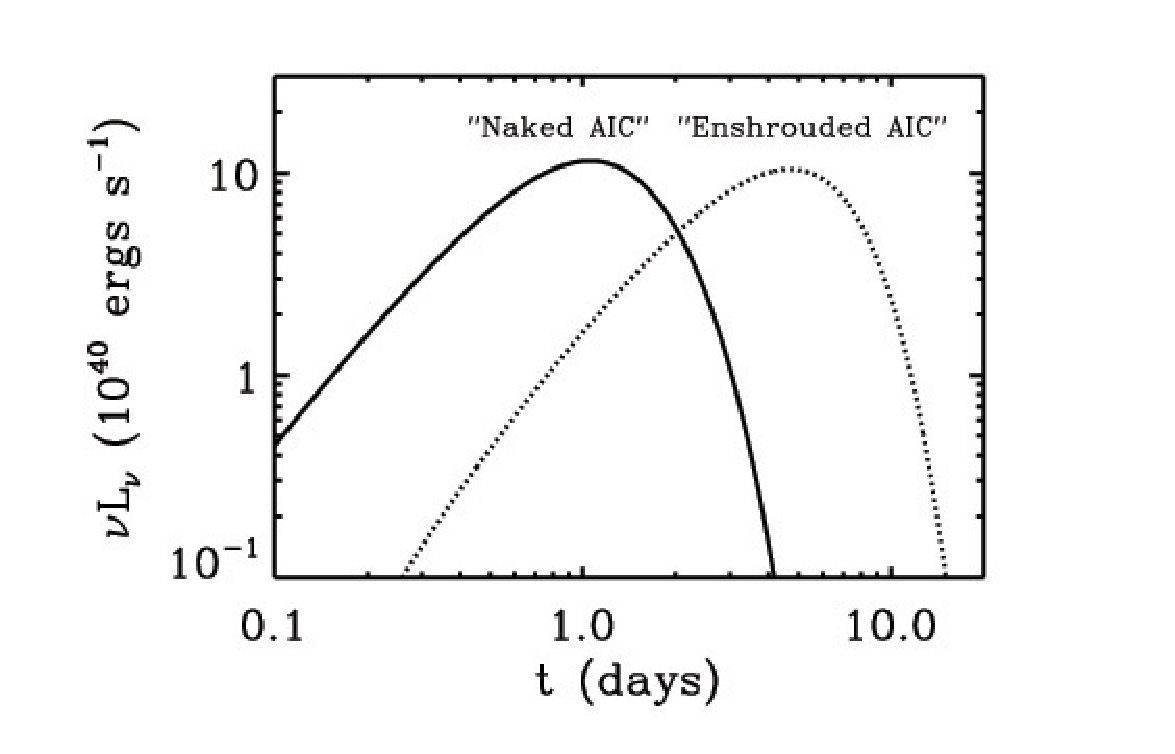
\includegraphics[width=0.8\hsize]{AICtrans.pdf}}
%\caption{Model V-band light curve of two AIC transients.  The naked transient (total mass $2 \times 10^{-2}$ {\Msun}, $10^{-2}$ {\Msun} $^{56}$Ni, $v = 3 \times 10^4 km s^{-1}$), resulting from a stable mass transfer AIC, does not have an envelope left over from a WD merger, and rises and falls within a day's time.  The enshrouded AIC transient (total mass $2 \times 10^{-1}$ {\Msun}, $10^{-2}$ {\Msun} $^{56}$Ni, $v = 10^4 km s^{-1}$) results from a WD merger, and therefore as an envelope that stretches out the light curve over a week while keeping peak luminosity constant.  These curves are consistent with \cite{frye+09}'s Fig. 7.  From \cite{metz+09}, their Fig. 2.}
%\label{AICtrans}
%\end{figure}

%SHOULD I USE FRYER'S INSTEAD - MORE BANDS??

%Such an ``enshrouded AIC'' transient could be responsible for SN 2008ha, whose rise time, peak luminosity, ejecta velocity, ejected mass and ejected {\Ni} are all within range of the corresponding values stated above.  With 0.16 {\Msun} ejected at speeds of $\sim 10^4$ km s$^{-1}$ and $\sim 0.02$ {\Msun} {\Ni} produced, and possible detection of Al II lines in its spectrum, SN 2010X is also an enshrouded AIC candidate \citep{kasl+10}.  It is not likely for this merger channel to explain all possible sub-luminous SNe Ia, as most others eject much more $^{56}$Ni than can be formed from an AIC-related transient \citep{fole+09}.

%If the WD merger remnant rotates differentially, then any initial poloidal magnetic field will be greatly amplified through the magnetorotational instability.  \cite{dess+07} show that the entire star consequently spins down by as much as 30\%, and the rotational energy lost is fed into a magnetically driven wind substantially more powerful than the neutrino wind described above.  Explosion energies then reach up to $\sim 10^{51}$ erg and $\sim$ 0.1 {\Msun} is ejected, though negligble amounts of {\Ni} are created.  The transient, therefore, is still fairly weak optically, and could instead be detected via neutrino and gravitational wave emission \citep{dess+07}.

%\citeauthor{metz+09} also speculate as to whether an AIC could emit a collimated relativistic outflow, thereby creating a short gamma-ray burst.  One advantage to AIC-GRBs is that the late-time (around 10 - 100 s) x-ray tail seen in some short GRBs could plausibly be explained by late-time accretion of merger remnant material not carried away by the initial AIC outflow, or by magnetar outflows (assuming one is created by an AIC).  See \cite{dess+07}, however, for discussion as to why AICs likely will not create short GRBs unless the collapsing WD eventually forms a black hole.  This 10 - 100 s x-ray emission might be seen regardless, and could be a target for x-ray survey missions \citep{metz+09}.

%%WHY IS TOTAL ENERGY GREATER IN ENSHROUDED CASE?

%%-Nucleosythetically speaking, could an ONeMg WD create an SN Ia?  I.e. the ejecta composition should be different, but in what way?  Fairly sure the answer's no - see Taubenberger on ONeMg explosion speculation.



%For a helium WD merging with a carbon-oxygen one, a helium giant could form, observable as a hydrogen-deficient giant or RCrB star.  

%For two carbon-oxygen WDs (CO WDs), the outcome could vary between simply a more massive WD, a carbon-burning star, an explosion, or collapse to a neutron star, depending on whether stable or unstable carbon fusion is ignited, and whether the total mass exceeds the critical mass for pycnonuclear ignition or electron captures (both close to the Chandrasekhar mass \Mch).  For mergers involving an oxygen-neon WD, the mass will always be high, and explosive demise or transmutation seems inevitable.


%%The merger of two white dwarfs (WDs) originally in a short-period binary is estimated (eg. \citealt{badem12}) to occur about once every century in a Milky Way-like galaxy, making the products of such events common throughout the universe.  They have been held responsible for producing a variety of stars with strange properties, including helium-burning sdOB stars \citep{saioj00, justph11}, RCrB stars (eg. \citealt{webb84, clay+07, clay13}), and massive and highly magnetized WDs (eg. \citealt{segrcm97, garc+12, kule+13}) that could resemble the hot DQ WDs (eg. \citealt{dunlc15}, Dunlap and Clements in preparation).  They may, however, also be responsible for spectacular transient events including accretion-induced collapses (eg. \citealt{saion85, abdi+10}) and type Ia supernovae (SNe Ia; eg. \citealt{howe11, hill+13, maozmn14}).  Determining the final outcome of a particular merger requires an understanding of the detailed dynamics of the merging process, which cannot directly be seen using current observational capabilities.  Thus, studies of merger physics have primarily utilized hydrodynamic simulations.
